%ब
\chapter{Proposed Solutions} \label{c:solutions}

This chapter describes the four  solutions proposed to implement referential
integrity constraints in a cloud \ac{NoSQL} \ac{DBMS}. 
Section~\ref{s:Metadata} describes some of the 
traditional approaches adopted to store  data dependency information in
popular \acp{RDBMS} and explains  the approaches of proposed solutions to store
the dependency information.  Section~\ref{s:API} describes the design and
implementation of the experimental API developed to integrate all the four
solutions. 
Section~\ref{s:sol1} describes how the first proposed solution implements
referential integrity constraints by saving metadata along with the actual data. 
Section~\ref{s:sol2} describes the second proposed solution where metadata
is saved as a top row and 
Section~\ref{s:sol3} describes the third  proposed solution of saving metadata
separate from the actual data to implement these constraints.  Finally, the
fourth solution of saving metadata in a separate cluster is described in Section~\ref{s:sol4} along with its implementation of the constraints. 

\section{Introduction}\label{Introduction-Solutions}
As mentioned previously, cloud column-oriented key-value \acp{DBMS} lack
referential integrity constraints to
maintain foreign key relationships as seen in traditional
\acp{RDBMS} due to its non-relational data model.  Moreover, these \acp{DBMS} do
not normalise data nor maintain relationships.  Traditionally, foreign key
relationships are maintained by correctly identifying and preserving the data
dependencies existing between data items in a database.  These dependencies
are maintained and  validated by imposing referential integrity constraints on
them. 

Most popular traditional \acp{RDBMS} preserve such dependency information
in their \texttt{System} tables or data dictionaries.  These tables store the
necessary information like the table
names, primary and foreign keys and so on that are required to maintain valid
dependencies. 
This can be seen in popular \acp{RDBMS} like  MS SQL Server, PostgreSQL,Oracle,
and so on.  For example, in MS SQL Server 2000, 
\texttt{sysforeignkeys}, one of the the \texttt{System} tables, stores the
information of all the foreign keys existing in the tables in a database and \texttt{sysreferences} stores the mappings of
the foreign keys to the referenced columns \citep{sys:msdn}. 
Information in these \texttt{System} tables consist of  the objectIDs of the
table with constraints, IDs of all the referenced and referencing columns, the
IDs of all the referenced keys and so on. In PostgreSQL, such information is saved
as views which contain the object dependency information for a database.  The
view \texttt{table\_constraints} contains the information for all the
constraints in a table belonging to the current user. (\todo{\cite{}}.  Similarly,
Oracle uses its \texttt{SYSTEM} meta-database to hold such information.  Such
\texttt{System} tables and views with information about the existing
dependencies  are looked up whenever referential integrity checks are triggered
\citep{sys:msdn}. 

In the proposed solutions  a similar approach is adopted where  all the
information about the data relationships between column families in maintain in
keyspaces and this information is looked up whenever referential integrity has
to be validated.  The dependency information is saved as metadata in all the
proposed solutions and  the following section describes how metadata is
modelled in these solutions. 

\section{Metadata}\label{s:Metadata}
Generally metadata is termed as data about data and 
commonly in \acp{DBMS}, metadata is holds the various information
about the contents of a database like schema details, constraints, information
about keys and so on.  As mentioned above, most traditional \acp{RDBMS}
maintain such metadata within their \texttt{System} tables or data dictionaries
where metadata is decoupled form the actual data and its operations  so that
retrieving the metadata is faster as it does not involve handling the actual
data. 

It has been studied that \ac{DaaS} is moving towards maintaining metadata in the
cloud \acp{DBMS}, where commonly this metadata stores information about the
nodes in the distributed cluster (\todo{cite Bin(2010)}).  For  maintaining the
scalability required in such cloud \ac{DBMS} metadata is often decoupled from
the actual data so that accessing metadata does not cause a bottleneck in
performance.  Cassandra maintains some metadata about each of the nodes in a
cluster separately in a \texttt{System} keyspace which stores the properties of
each node in a cluster like its node token, the name of the cluster the node
belongs to,information about the stored keyspaces and column families and so
on(\todo{cite BOOK}). 

As per the design of Cassandra, the \texttt{System} keyspace cannot be modified
and thus  the metadata for the proposed solutions cannot be incorporated in this
\texttt{System} keyspace.  Hence, for preserving the metadata in the
proposed solutions, different strategies were designed
and each design was implemented as a separate solution.  This meant metadata had
to be associated with actual data in different ways.  According to Duval
(\todo{cite}), such associations can be of three kinds, namely:

\begin{itemize}
  \item Embedded Metadata - is the metadata that is created when the data is
  created by the user.  Hence, metadata is embedded within the actual data
  itself. 
  \item Associated Metadata -  is the metadata that is preserved separate from
  the actual data and changes to the metadata does not involve handling the
  data. 
  \item Third-party Metadata- is the metadata that is maintained by a third
  party like a cloud service provider and the metadata is separately stored from
  the actual data. 
\end{itemize}
Both associated metadata and third-party metadata require mechanisms for
managing  data and its metadata correctly and efficiently.  In most applications,
metadata is stored separately from actual data when the actual data is large
and interconnected and generally metadata is accessed frequently.  To prevent
bottlenecks metadata is stored separately from the actual data so that
metadata retrieval is easier and does not involve operations on the actual
data. 

In the proposed solutions, Solutions 1 and 2  use embedded data while Solutions
3 and 4 use associated metadata.  The structure of the metadata is kept the same
across all the solutions to maintain consistency in processing metadata and the
validation of referential integrity in all the solutions.  

The role of metadata in all the solutions is primarily to hold the necessary
 information required to maintain referential integrity like information about
 primary keys, foreign keys, referenced and referencing column family details
 and so on so that this metadata can be accessed whenever a referential
 integrity validation is triggered in the solutions.  
In the solutions, existing constraints which can be either \ac{PK} constraints
or \ac{FK} constraints are saved as metadata.  A \ac{PK} constraint specifies
which column is the primary key in a column family.  A \ac{FK} constraint
describes the foreign key relationship between two column families where a
column of one column family will be dependent on the primary key column of another
column family.  Hence, if \texttt{10} column families with primary keys exist in
a keyspace, then the metadata will contain \texttt{10} \ac{PK} constraints saved
as metadata and any foreign key relationships would be saved as \ac{FK}
constraints. 

 Throughout the solutions,
 the structure for these constraints saved as metadata  is consistent while
 the way of storing and associating this metadata is different
in each solution.  The general structure of the metadata is shown in
Figure~\ref{f:meta-struc}. \\

\begin{figure}[h]
	\centering
	%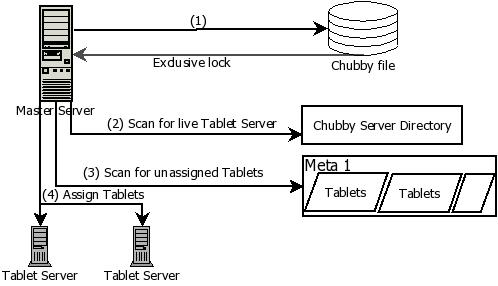
\includegraphics[width=5cm,   height=5cm]{.  /figure/random.  jpg}
% 	
\includegraphics[width=1. 1\textwidth]{. /figure/Solutions/Metadata-Structure. png}
	\newcolumntype{C}{@{\hspace{2pt}}>{\bfseries\scriptsize}c@{\hspace{2pt}}|}
	\begin{tabular}{|CCC CCC CC}
		\hline
		ConstraintName & Keyspace & ConstraintType & ColumnFamily & RKeyspace &
		RConstraintName & RColumn & DeleteRule\\
		\hline
	\end{tabular}
	\caption{Structure of Metadata in the Solutions}\label{f:meta-struc}
\end{figure}


 The above illustrated structure applies to every
constraint and each part of this structure represents information about the
constraint. This structure is described below using the University
keyspace example, which was explained in Section~\ref{s:key-value-data-model}
and illustrated  in Figures~\ref{f:meta-pk}
and \ref{f:meta-fk}. 

\begin{itemize}
  
  \item \texttt{ConstraintName:} is the name or a  Unique ID assigned for every
  constraint saved as metadata and it uniquely identifies an
  existing \ac{PK} and \ac{FK} constraint in the metadata. 
  For example,in the Figures~\ref{f:meta-pk} and
  \ref{f:meta-fk}, \texttt{CONST100} and \texttt{CONST400} are the \texttt{ConstraintNames}. 
    
  
  \item \texttt{Keyspace:}represents the name of the Keyspace the constraint
  belongs to. 
  In Figures~\ref{f:meta-pk} and \ref{f:meta-fk}, both constraints belong to the
  keyspace \texttt{University}. 
  
  \item \texttt{ConstraintType:}denotes the type of the constraint.  '\texttt{P}'
  denotes that it is a \ac{PK} constraint and '\texttt{R}' denotes that it is a
   \ac{FK} or referential integrity constraint. 
   
 
  
  \item \texttt{ColumnFamily:}refers to the Column family this constraint
  exists in. 
  In the example,  Figure~\ref{f:meta-pk} shows the primary key constraint
  existing in column family \texttt{User} and the column family for the foreign
  key constraint in Figure~\ref{f:meta-fk} is \texttt{Enrolment}. 
  
  \item \texttt{RKeyspace:}is the name of the keyspace on which this constraint
  is applied.  In Figures~\ref{f:meta-pk} and \ref{f:meta-fk}, both constraints
  are applied in  the keyspace \texttt{University}.  If these constraints were
  applied on column families existing in a foreign keyspace like a
  \texttt{HealthService} keyspace, it would contain the name of the foreign
  keyspace. 
  
  \item \texttt{RConstraintName:}In the case of a \ac{FK}
  constraint, \texttt{RConstraintName} represents the name of the \ac{PK}
  constraint that is referenced by this \ac{FK} constraint.  This referenced
  \ac{PK} constraint indicates which primary key column  is being referenced
  by this \ac{FK}.  constraint.  In Figure~\ref{f:meta-fk}  the \ac{FK}
  constraint \texttt{CONST400} is referencing the
  \ac{PK} constraint 
  \texttt{CONST100}, which points to the primary key for the \texttt{User}
  column family.  This shows that \texttt{Enrolment} has a foreign key
  relationship with \texttt{User}.  In a Primary key constraint, it is left blank
  as it does not reference any other constraint, as seen in Figure~\ref{f:meta-pk}. 
  
  \item \texttt{RColumn:}  indicates the primary key column on which this
  constraint is applicable.  For \ac{PK} constraints, this holds the name of
  the primary key column.  For example, in Figure~\ref{f:meta-pk} this shows that
  the \ac{PK} constraint is applied on the primary key column \texttt{UserId}. 
  
  For \ac{FK} constraints this field denotes the referenced column.  In
  Figure~\ref{f:meta-fk}, this means that the referenced column is
  \texttt{UserId}, indicating that \texttt{Enrolment} references
  primary key column \texttt{UserId} of \texttt{User}. 
  
  \item \texttt{DeleteRule:}stores the type of data manipulation rule applicable
  on this constraint like Cascade or NoDelete. 
  
\end{itemize}


\begin{figure}[h]
	\centering
	%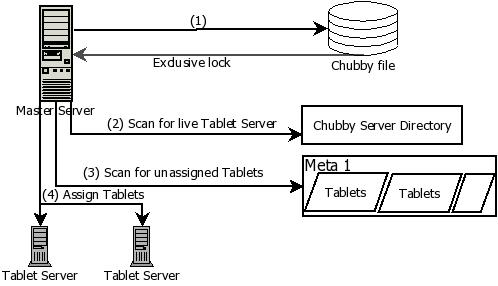
\includegraphics[width=5cm,   height=5cm]{.  /figure/random.  jpg}
% 	
\includegraphics[width=. 6\textwidth]{. /figure/Solutions/Metadata-PK}
\newcolumntype{C}{@{\hspace{2pt}}>{\scriptsize}c@{\hspace{2pt}}|}
	\begin{tabular}{|CCC CCC CC}
		\hline
		\bfseries ConstraintName & \bfseries Keyspace & \bfseries ConstraintType &
		\bfseries ColumnFamily & \bfseries RKeyspace & \bfseries RConstraintName &
		\bfseries RColumn & \bfseries DeleteRule\\
		\hline
		CONST100 & University & P & User & University & & UserId &\\
		\hline
	\end{tabular}
	\caption{Metadata for a Primary Key in the Solutions}\label{f:meta-pk}
\end{figure}


\begin{figure}[h]
	\centering
	%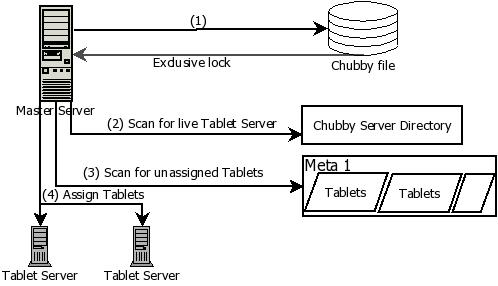
\includegraphics[width=5cm,   height=5cm]{.  /figure/random.  jpg}
% 	
\includegraphics[width=. 78\textwidth]{. /figure/Solutions/Metadata-FK}
\newcolumntype{C}{@{\hspace{2pt}}>{\scriptsize}c@{\hspace{2pt}}|}
	\begin{tabular}{|CCC CCC CC}
		\hline
		\bfseries ConstraintName & \bfseries Keyspace & \bfseries ConstraintType &
		\bfseries ColumnFamily & \bfseries RKeyspace & \bfseries RConstraintName &
		\bfseries RColumn & \bfseries DeleteRule\\
		\hline
		CONST400 & University & R & Enrolment & University & CONST100 & UserId &
		CASCADE\\
		\hline
	\end{tabular}
	\caption{ Metadata for a Foreign Key in the Solutions}\label{f:meta-fk}
\end{figure}

% Metadata can be associated with real data in three ways according to \todo{cite
% Duval}:
% \begin{itemize}
%   \item Embedded Metadata - is the metadata that is created when the data is
%   created by the user. 
%   \item Associated Metadata -  is the metadata that is preserved separate from
%   the actual data and changes to the metadata does not involve handling the
%   data. 
%   \item Third-party Metadata- is the metadata that is maintained by a third
%   party like a service provider. 
% \end{itemize}
% Both associated metadata and third-party metadata required mechanisms for
% managing both data and its metadata correctly and efficiently.  In most cases
%metadata (\todo{cite Duval}). 

% Based on these ways, it can be inferred that the proposed solutions involve both
% embedded metadata in Solutions 1 and 2 and associated metadata in Solutions 3
% and 4.  The structure of the metadata is kept the same across all the solutions
% to maintain consistency in processing metadata and the validation of referential
% integrity in all the solutions. 
Metadata in the solutions are accessed whenever referential integrity
validations are triggered so that information about \ac{FK} constraints are
extracted.  Specific methods are designed in all the solutions to read and
process the metadata so that referential integrity can be validated.  These
methods and all the solutions are incorporated into a single \ac{API}, which is
described below. 

\section{Experimental API}\label{s:API}
While designing the \ac{API}, much attention was paid to ensure that it can be
used by most applications to maintain dependencies within its keyspace
irrespective of the keyspace schema or structure of the column families. 
The users of this experimental \ac{API}  have to provide the metadata
information relevant to their keyspace like the existing \ac{PK}
and \ac{FK} constraints in the column families which they want to maintain
within the keyspace. 
Thus, this \ac{API}
is made adaptable to different keyspace schemas  that can be deployed in
column-oriented key-value \ac{DBMS}.  For example, user applications could use
this \ac{API} to maintain referential integrity in a keyspace that is modelled
to store information about a University or a Hospital or other entities.  

This \ac{API} validates the referential integrity based on the metadata provided
by the user application for its column families.  The \ac{API} provides the user
applications with the four solutions using which users can save their metadata
information in a particular way like embedded or associated and they can use the
solutions to impose referential integrity validation.  All the solutions adopt
the same design patterns and their implementation is also the same. 

%  The University
% example assumes that students enrol into different courses and student
% information is saved in the \texttt{Student} column family, the course data in
% \texttt{Course} column famil and their foreign key relationship in
% \texttt{Enrolment} This example is illustrated in
% Section~\ref{s:key-value-data-model}.  Figure~\ref{} presents the class diagram
% followed during the design of \ac{API}. 

The main components of this \ac{API} and the basic operations it provides like
\ac{CRUD} are described below.  The column families and the
dependency information will be different for different user applications.  Hence,
a general class diagram for this \ac{API} is given in
Figure~\ref{}. 
\\
\todo{Insert class diagram- not university entities}

	\subsection{Entities} 
	Generally, an entity represents a real world object which has attributes
	associated with it and it is defined during the conceptual data modeling of
	data as in the popular \ac{ER} model\todo{cite navathe}). .  
	In most applications, an entity is commonly considered as a \ac{Pojo} and an
	instance of an entity refers to a single record in a table.  This is similar in
	the \ac{API} as well, where entities are  represented as column families and
	every instance of an entity  denotes a super column in the column family. 
	For example, in the University keyspace example,an entity can be 
	\texttt{Student} and its instances will be the  super columns in
	\texttt{Student}. The columns in the column family can
	be considered as the attributes of the entity instances. Some of the other
	entities for this example are \texttt{Course} and \texttt{Enrolment}. 
	
	In the \ac{API}, entities of  user applications are
	designed to extend the abstract class called \texttt{BaseEntity}, which has methods for
	accessing and defining the entities.  This is applicable to all the four
	solutions under this \ac{API}.  By extending the \texttt{BaseEntity}, all user
	applications using this \ac{API} have to implement these methods for retrieving
	or defining the entities and this procedure ensures that all applications adopt the same ways
	to do so.  The operations that can be performed on these entities like
	\ac{CRUD} operations are handled by an \texttt{EntityManager}, which is
	described in the following subsection. 
	
	\subsection{EntityManager}
	Generally, when any application connects to a database a session is maintained
	while the database connection lasts.  Generally, during such sessions applications maintain
	a persistence context which is a cache to store the state information of
	entities retrieved from the database, so that the database is not directly
	accessed for every operation on an entity (\todo{apachetomee, javadoc}). 
	Commonly the persistence context is accessed through an interface called
	\texttt{EntityManager} that provides the basic \ac{CRUD}
	operations to access data.  Such an approach is adopted by the proposed \ac{API} where the
	\texttt{EntityManager} is called \texttt{BaseDAO}.  
	
	However, it
	is complex and computationally expensive to maintain such a persistence context
	for applications using cloud \acp{DBMS} since entities are replicated on many
	nodes with the possibility of many users concurrently accessing and changing its
	state.  In such a dynamic environment, maintaining the persistence context
	becomes an overload for applications as it has to
	 connect to the underlying \ac{DBMS} often and ensure that the entities are
	 always up to date. 
	 
	Hence, the \texttt{BaseDAO} for all the solutions of this \ac{API} connects to
	the keyspace directly and avoids the overhead of maintaining such a persistence context. 
	\texttt{BaseDAO} accesses a keyspace by connecting to one of the nodes in the
	cluster and handles all the \ac{CRUD} operations performed on the entities in the
	\ac{API}. These operations trigger some referential
	integrity validation on entities and follows the
	referential integrity rules which were described in
	Section~\ref{s:referential-integrity}. 
	The implementation of these operations in the \ac{API} are described below.   % 
	% An
	% \texttt{EntityManager}
% 	represents the session an application maintains with the database.  It is
% 	basically the interface to access and interact with the persistence context,
% 	which in simple terms is the cache of data retreived from the database.   Such a
% 	persistence  context helps as the numebr of times a database has to be directly
% 	accessed is reduced and instead a copy of the data persists in the memory and is
% 	used in the necessary operations required by the application, thus recuding the
% 	consumption of many resources. This persistence context has a set of entity
% 	instances along with a set of operations to interact with these instances of
% 	data. 
		
% 	Generally, applications that handle data in a database use an
% 	\texttt{EntityManager} to access the underlying database, which performs the
% 	correct operations on the entities in the persistance context and these
% 	operations are commited into the database once a transaction is committed.  
%  	.  
 	 
	
		\subsubsection{Create}
		In an \texttt{insert} operation, entities provided by the
		user application are read by the \ac{API} and these are passed as parameters to the
		\texttt{BaseDAO}.  The \texttt{BaseDAO} inserts these entities into the column
		families the entity belongs to.  For example, all the student records are
		inserted into the column family \texttt{Student} through the \texttt{BaseDAO}. 
		
% An \texttt{insert} operation inserts an entity into the database and commits
% it. 
		In the proposed \ac{API} this operation triggers a referential integrity
		validation whenever a child entity is  inserted since a child entity contains
		the foreign keys of its parent entities.  Based on the referential integrity
		\texttt{insert} rule,  valid parent entities with primary keys matching these
		foreign keys must exist. , else  an exception is raised stating that the
		referential integrity has been violated.  
		The implementation of the \texttt{insert} operation is consistent across all
		the solutions. 
		
		
		User application provides the metadata pertaining to their keyspace and this is
		inserted using this \texttt{insert}operation through the \texttt{BaseDAO} in
		all the solutions. 
% This
% 		metadata also contains the data manipulation rule applicable for each entity,
% 		like \texttt{Cascade} or \texttt{NoDelete}.  This is necessary for the
% 		\texttt{Update} and \texttt{Delete} operations. 
		
		\subsubsection{Read}
		In a \texttt{Read} operation  entities are identified and retrieved by its
		key. 
		In the proposed \ac{API}, this operation does not prompt any referential integrity
		validation since entities are only read and their state is not changed 
		 unlike in other operations. 
		Every time entities are inserted, updated or deleted, the \texttt{Read} operation is
		initiated by the \texttt{BaseDAO} to retrieve the correct entities on which
		these operations are to be executed. 
		The keys of the entity instances that have to be read are passed form the
		solutions to the \texttt{BaseDAO} and it in turns retrieves these entity
		instances or the relevant super columns from the column families.  The
		\ac{API} supports reading  all the instances of an entity from its column family or a
		single entity by providing its key. 
		
		
		\subsubsection{Update}
		In an \texttt{update} operation the existing state of an entity is merged
		with a new state provided by the user application. 
		This means that  values of columns are updated to new values and these are
		committed into the column families by the \texttt{BaseDAO}.  The
		\texttt{BaseDAO} receives the entity and the new values provided by the user
		application and commits the changes to the column family of the entity. 
		
		In all the solutions, an \texttt{Update} operation triggers a referential
		integrity validation and follows the referential integrity \texttt{update} rule  whenever
		any child or parent entities are updated.  
		
		When a parent entity is updated on its primary key column,  the
		\texttt{BaseDAO} checks the metadata to locate  any existing constraints on
		this parent entity.  If dependencies are found then, based on the parent
		entity's \texttt{DeleteRule}, the child entities are either updated or the
		operation is cancelled.  If the \texttt{DeleteRule}  is \texttt{Cascade}, or
		is \texttt{NoDelete} but has no current child dependencies, then the child 
		entities are correctly updated prior to updating the parent entity's primary
		key column.  If the \texttt{DeleteRule} is \texttt{NoDelete}, with existing
		child dependencies, the \texttt{update} operation is prevented and an
		exception is raised.  For example, in the University keyspace example, when a
		new \texttt{UserId} is provided for an existing  \texttt{Student}
		instance, then \texttt{BaseDAO} checks metadata and locates the \ac{FK} constraint
		\texttt{CONST400} as seen in Figure~\ref{f:meta-fk}.  Since the
		\texttt{DeleteRule} is \texttt{Cascade}, all the old \texttt{UserId} values
		for this \texttt{Student} instance in \texttt{Enrolment} are updated with the new
		\texttt{UserId} values prior to updating the \texttt{Student} instance. 
		
		When a child entity is updated on any of its
		foreign key columns, the \texttt{BaseDAO} performs the same check on the
		metadata and locates its parent entities and the referenced primary key columns. 
		If the new values of the foreign keys are not present as a primary key for any of the
		parent entities, then an exception is raised and this update is prevented,
		otherwise, the update is performed.  For example, when the foreign key
		\texttt{UserId} for one of the instances of \texttt{Enrolment} is given a new
		value, then the \texttt{BaseDAO} identifies the parent entity for this
		\ac{FK} constraint as \texttt{Student}.  If the new
		\texttt{UserId} exists as a primary key for any of the \texttt{Student}
		entities, the \texttt{update} is performed. 
		
% 		To locate the references in the metadata as well as locating the correct
% 		entities and its columns, the \texttt{BasDAO} performs the \texttt{Read}
% 		operations. 
		The \texttt{BaseDAO} reads the metadata and the entities and their keys using
		the \texttt{read} operation. 
		
		\subsubsection{Delete}
		In a  \texttt{Delete} operation entities to be removed from a column
		family are sent to the \texttt{BaseDAO}. 
		I all the solutions, a \texttt{Delete} operation triggers a referential
		integrity validation and follows the referential integrity \texttt{delete}
		rule every time a parent entity is deleted.  To validate referential integrity,
		the \texttt{BaseDAO} performs a \texttt{read} operation on the metadata and 
		locates if the entity
		marked for deletion has any existing \ac{FK} constraints that depends on the
		entity's primary key. 
		
		If the parent  entity has a \texttt{Cascade} rule, or has a
		\texttt{NoDelete} rule with no current dependencies, then the child entities
		are deleted prior to deleting the parent entity. 
		
		For example, in the University keyspace, if a 
		\texttt{Student} instance is marked for deletion, then the \texttt{BaseDAO}
		locates the child entities that are referencing \texttt{Student} like
		\texttt{Enrolment} from the constraint \texttt{CONST400}
		(Figure~\ref{f:meta-fk}).  Since the \texttt{DeleteRule} is \texttt{Cascade},
		the child entities are deleted from \texttt{Enrolment} prior to deleting the
		\texttt{Student} instance. 
		
		\subsection{ValidationHandler}
		The \texttt{ValidationHandler} is invoked by the \texttt{BaseDAO} every time
		an operation like \texttt{insert}, \texttt{update} or \texttt{delete}, triggers a
		referential integrity validation on any entity. 
		The \texttt{BaseDAO} passes the entity, its
		column family information and its metadata  to the
		\texttt{ValidationHandler} to perform the validation.  
		
		The	\texttt{ValidationHandler} contains the logic for checking whether the entity
		has any dependencies and decides whether the operation violates the
		referential integrity or not.  For example, in the University keyspace if the
		new foreign key \texttt{UserId} for an \texttt{Enrolment} entity does not
		exist as a primary key for any of the \texttt{Student} instances,  the
		\texttt{ValidationHandler} signals \texttt{BaseDAO} to raise an exception and
		to abort the operation.  The	pseudocode for validating the referential
		integrity in an \texttt{Update} operation is shown in
		Figure~\ref{f:VHpseudocode}. 
		(\todo{Change to text later}) \begin{figure}[h]
			\centering
			%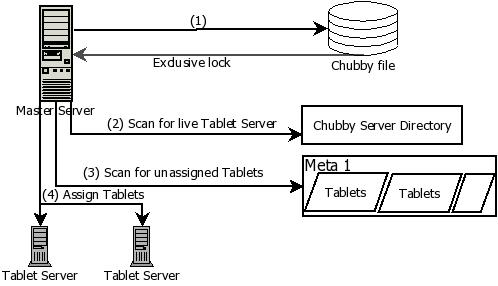
\includegraphics[width=5cm,   height=5cm]{.  /figure/random.  jpg}
			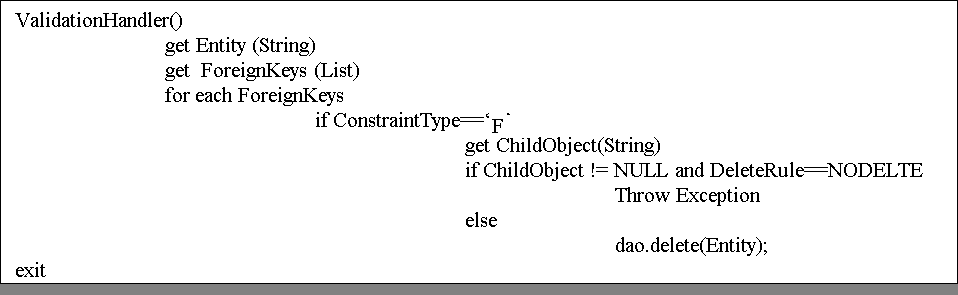
\includegraphics[width=.8\textwidth]{./figure/Solutions/VH-UpdatePseudocode.png}
			\caption{\texttt{ValidationHandler} Pseudocode for an
			\texttt{Update} operation}\label{f:VHpseudocode}
		\end{figure}
		
		Since the way metadata is stored in the solutions are different, the
		\texttt{ValidationHandler} will be slightly different for each solution in the
		\ac{API}.  For example, the \texttt{ValidationHandler} for Solution 1 and 2
		involves parsing the metadata since it is stored as a
		\texttt{String} along with the actual data. 
		
		\subsection{Connection to Cassandra}
		In the experimental \ac{API}, an operation  performed on entities requires
		accessing a column family belonging to a keyspace in Cassandra.  To establish a
		connection to a Cassandra cluster, so as to access keyspaces and to complete
		the operations, the experimental \ac{API} uses one of the early client \acp{API}, Hector.  Hector is a high level client that wraps the driver-level interface of Cassandra called Thrift
		and provides more benefits than Thrift like fail-over mechanisms and
		connection pooling (\todo{cite book}).  Hector was the chosen \ac{API} for this thesis
		since using hector it was possible to bypass interacting with Thrift.  The
		learning curve to understand and use Thrift proved to be steep and time
		consuming, considering the scope of the thesis. 
		
		To connect to a keyspace, \texttt{BaseDAO} creates a connection object for
		each of the solutions using Hector's  connection manager and this connection
		is used for all the operations on the entities.  To perform all the \ac{CRUD}
		operations on the entities, \texttt{BaseDAO} connects to the keyspace and uses
		Hector's methods to commit these changes to Cassandra.  
		
		While inserting	entities, Hector methods like \texttt{createStringColumn()},
		\texttt{createKeyspace} and so on are used by the \texttt{BaseDAO} to create
		columns and keyspaces based on the data supplied by the user
		applications.  For all operations \texttt{BaseDAO} creates a \texttt{Mutator}
		object defined by Hector, to insert, update or delete an entity in the
		cluster.  For example, in an \texttt{insert} operation, \texttt{BaseDAO} passes
		the entity details like its key and column family to \texttt{addInsertion} method of the
		\texttt{Mutator}. Similarly, \texttt{delete} method of \texttt{Mutator} is used
		for \texttt{BaseDAO's} \texttt{delete} operations. 
		
		The implementation, connection settings and accessing Cassandra through Hector
		is common for all the solutions in the \ac{API}.  As mentioned previously,
		solutions vary in the way they preserve metadata. 
		The following sections describe the solutions, the motivation for the
		solution's design and the way the solutions save metadata. 
		
% 	, except that all the operations
% 	are directly sent to the database through one of the \acp{API} provided by
% 	Cassandra.  This is because  Cassandra does not perform transactions as seen in
% 	\acp{RDBMS}, but rather operations on data at a time (\todo{cite}). 
% 	\texttt{BaseDAO} 
	
\section{Solution 1:  Metadata with Special Characters}\label{s:sol1}
% In RDBMSs, referential integrity constraints are enforced at the creation of
% tables (or updated later using ALTER TABLE).  In the above example, imposing
% the referential integrity constraint for the Enrolment table (Figure 3) would
% be using "FOREIGN KEY CourseID REFERENCES Course (CourseID)".  This would
% indicate that the CourseID of Enrolment table is dependant on the CourseID
% primary key of the Course table. 
	Much research has been done in the area of  metadata management in distributed
	environments  where emphasis is laid on the synchronous updates of metadata
	storage as well as its efficient storage and access mechanisms(\todo{cite more}
	Hackl et al.  2010). 
	In Hackl et al.  (2010)  metadata management is discussed in the context of huge
	file systems where metadata is stored separately in a suitable \ac{DBMS} so
	that such file systems can be managed and administered efficiently without
	slowing them down.  To analyse which type of \ac{DBMS} was more suitable for such a
	metadata storage, they conducted various experiments and concluded that
	key-value \acp{DBMS} were more efficient in terms of speed, memory and resource
	consumption when compared to popular \acp{RDBMS}.  As a part of their
	experiments,they adopted an interesting approach to store metadata in a
	key-value \ac{DBMS} , namely Tokyo Cabinet, a popular \ac{NoSQL} \ac{DBMS}. Tokyo
	Cabinet is a simple database library that stores records as simple key-value
	pairs in data files and unlike Cassandra does not involve data types or columns
	and so on.  In their approach, metadata about the file system used in their
	experiment is inserted as a value which is associated with a unique key and the
	different parts of the metadata are separated by semicolons (Hackl et al.  2010). 
	
	The first solution proposed in this thesis is inspired by this design of saving
	metadata as the value in a key-value pair and can be considered in
	column-oriented key-value \acp{DBMS} as well. 
	The solution proposes saving the dependency information of the entities as
	metadata and including this metadata in the entity's value.  In this solution,
	the metadata contains  various information related to the relationship between
	entities Figure~\ref{f:meta-struc}.  The  different parts of the metadata like
	\texttt{ConstraintName}, \texttt{RColumn}, \texttt{RConstraintName} and so on
	will be separated by a special character like a comma. 
	To achieve this in a column-oriented key-value \ac{DBMS} the metadata is saved
	as a part of each of the super column (or row) in a column family. 
	In every super column, this metadata is separated from the columns
	 by storing the metadata surrounded with curly brackets. For example, in the
	 University keyspace example, the column family of \texttt{Student} would save
	 the dependency information as a part of the value itself for every  super
	 column in it (Figure~\ref{}). 
	
	For this solution, the metadata is
	parsed by the \texttt{ValidationHandler} and  the different parts of the
	metadata are extracted to identify whether the entity has any dependencies.   
	Each constraint in the metadata is handled as a
	\texttt{String} and the special characters like '\texttt{\{}', '\texttt{,}'
	become the delimiters for parsing the \texttt{String} and splitting it into tokens.  
	Thus, each of these tokens
	would hold one of the parts of the constraint like \texttt{RColumn},
	\texttt{DeleteRule} and so on. 
	When foreign key relationships are found by the
	\texttt{ValidationHandler} after parsing the metadata for an entity, the
	appropriate actions are triggered like throwing an exception thus preventing the operation 
	or allowing the operation to execute. 
	
	In this solution,the metadata is saved  when entities are inserted into the
	column family and thus the metadata is a part of each of the entity.  Since the
	metadata is present as the value in every super column, accessing the metadata
	information for referential integrity validation is as simple as accessing the
	value itself, requiring no additional actions or connection to the keyspace
	
	On the other hand, the metadata for an entity would be the same for all the
	instances of the entity.  For example, in the University example, the metadata
	information for the \texttt{Student} entity is applicable to each of its
	instances, indicating that each instance  should have a primary key called
	\texttt{StudentID}. 
	Similarly, all \texttt{Course} instances have the same \ac{PK} constraints
	applied on it.  When metadata is saved as a part of the  value,
	every instance of an entity will contain the constraint information
	in it's value.  Since the metadata information and constraints are same for all
	the instances of a single entity , the metadata is repeated every time an
	instance of the entity is inserted.  For example, if 
	\texttt{1000} \texttt{Student} instances are inserted, the metadata for these
	\texttt{1000} instances are saved \texttt{1000} times too along with these
	instances.  But the metadata is exactly same for all the
	instances \todo{(Figure~\ref{})}. 
	
	Saving the metadata as embedded metadata helps when 
	entities are replicated across the distributed cluster, so that every node in
	the cluster contains the metadata information saved along with the entity.  The
	\ac{API} parses the metadata of an entity by reading any of its instances and
	need not load metadata from any external location. 
	The distributed nature of cloud \ac{NoSQL} \acp{DBMS} also means that the
	metadata is not only repeated several times within the same column family, but
	also across the nodes in the cluster,thus increasing the redundancy of
	the metadata.  But such a redundancy and consumption
	of space to store the metadata is not a potential issue in cloud column-oriented key-value \acp{DBMS} since storage on the cloud is inexpensive and thus does not affect the economic benefits either. 
	
	Such a storage mechanism is not expected to affect the efficiency of the
	cluster negatively as the metadata information is not large in size and is
	easily replicated along with the actual data and does not exert any extra
	resources in the cluster.  The performance of this solution is analysed  in
	Chapter~\ref{}. 
	
	
	
\section{Solution 2:  Metadata as Top Row}\label{s:sol2}



\section{Solution 3:  Metadata Tables}\label{s:sol3}



\section{Solution 4:  Metadata Clusters}\label{s:sol4}



